\documentclass[main.tex]{subfiles}

\begin{document}
\section{Control System Design Methodology}
\textit{This section covers Design methodology for control systems and software design. The focus is on the \gls{scada} architecture, how it is constructed and the methodology behind creating such a system. Finally, a discussion is made on the methodology of software design and common ways to structure code.}

Control systems have been a part of the industry for decades, and it started in 1960s, where specialized minicomputers interfaced directly with devices in the plant or factory\cite{scada_history}. These systems were primarily used used for automation, but they were highly specific and integrated to its system, using proprietary communication protocols and technology. Later, programmable controllers were starting to phase out minicomputers and \gls{hmi} have evolved from terminal with keyboards, to advanced \gls{gui}s. Ethernet eventually became the industry standard communication protocol. These technologies converged to a single system, such as system was nicknamed \gls{scada}.

The Readout units and the power supply board both require a software end point that essentially controls the entire system. This entails creating a system that can setup and configure the various parts of the system and also monitoring the system and report errors, i.e. we need to create a monitoring and configuration system.

A control system is generally is made out of sensors, a controller to control and retrieve data from the sensors, a supervisory computer that manages the process for the sensors, and \gls{hmi} software. The \gls{hmi} software provides access to the data from the sensors to the user and if needed, also allow the user to modify processes in the system.


\subsubsection{SCADA systems}
 \gls{scada} systems have five main functions: data collection, network data communication, data presentation, and remote monitoring and supervisory control\cite{scada_intro}. Although today, many control systems is based on \gls{iot}, which has a similar architecture. However, \gls{iot} bases itself on utilizing cloud-networking and processing for its communication infrastructure. Due to lack of wireless communication in the \gls{pct}-project, focus will be on how \gls{scada} systems are developed, although many of the same principles applies for both.

A \gls{scada} system typically is made out of five components:

\begin{itemize}
    \item Field devices and signals
    \item \acrfull{ppc}
    \item \acrfull{hmi}
    \item Database servers
    \item Communication infrastructure
\end{itemize}

Field devices and signals encompasses all sensors and the actuators that controls them. \gls{ppc} is responsible for automatically controlling the field devices, as well as retrieving data from them and send it to the \gls{hmi}. A microcontroller is an example of a \gls{ppc}. \gls{hmi} is the software being executed on the main computer and is made of a user interface and database manager. The \gls{hmi} serves as the interface for the user to set up configuration processes and monitor the system performance. For this purpose, a configuration database is required to set up the \gls{ppc}s with correct values, and a historical database is needed to store monitoring data from the field devices. A communication infrastructure connects the \gls{ppc}s to the workstations running the  \gls{hmi} software.

\subsubsection{Communication network}
There are various communication networks that can be used in a \gls{scada}-system, since all data from the sensors in the \gls{pct} project comes from IPbus, it makes sense for one master computer to receive the data from the IPbus and process it, or send to other computers for processing. (McCrady, 2013) describes in his book of such a communication topology\cite{scada_design}. An example of a \textit{star} topology is shown in \autoref{fig: scada_star}.

\begin{figure}[!ht]
    \centering
    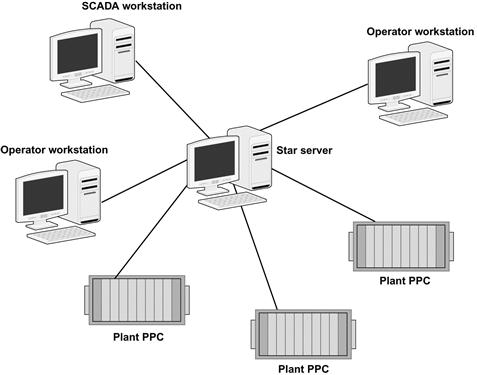
\includegraphics[scale=0.6]{images/scada_topology.png}
    \caption{Example of a star topology communication infrastructure used for SCADA systems\cite{scada_design}}
    \label{fig: scada_star}
\end{figure}
\FloatBarrier

In the \gls{pct}-project, the main computer can be connected to readout, power delivery, and cooling, leading to a \textit{star} topology, even if no other computers are connected.

\subsubsection{I/O Signals}

Important in a \gls{scada} system is to identify all signals to be used and retrieved by the field devices. Knowing all signals to be used in a system will give us an estimate of the requirements of the system as well as aid in the development process.

Power delivery uses a microcontroller to manage power output as well as temperature of the sensors. The microcontroller measures analog voltage(AVDD), digital voltage(DVDD), PWELL voltage, and the temperature of strings. It also have two register for each measurement that dictates the threshold levels, which will make the microcontroller turn off the power if these levels are exceeded. if we include monitoring an error register, and configuring enable signals for the strings, it will then result in 8 input/configuration signals and 8 output/monitoring signals.

\notinmain{Skriv meir om readout og cooling I/O signaler her, ha med ein tabell og kanskje}

\subsubsection{Software documentation}
Another important aspect of such a control system is having a consistent programming standard and complete software documentation. \gls{scada} and similar systems often have a long shelf time, and a well documented system will make maintenance and work in the future be much easier. In general, starting with good software documentation and expanding upon it during the project development will lead to sufficient documentation of the entire system.

A consistent programming standard helps in debugging and in expanding functionality of the system. \gls{oop} is a very common programming paradigm that is used to give structure to programs and increase reusability and maintainability of the code. Systems designed to manage large data acquisition, such as a \gls{pet}-scan system, have in the past used \gls{oop} to design and manage large programs\cite{pet_control_system}, this suggest that this programming structure is viable for the design of the control system in the \gls{pct}-project.



\subsection{Git and GitHub}

The use of the Git and GitHub tools is essential today to manage your code, maintain it and also as a version control system. Git is another method used to ensure that the code is easy to use and be maintained, now and in the future. The version control system is also essential for verifying the code, mistakes can be made, but a stable version of the software will always be available at the GitHub. GitHub also enables a better workflow with co-developers or mentors, allowing easy access to the source code and issues can be made. There is currently only one master branch of the repository in the Git system, this is due there only being one developer so branching is not yet needed.

The GitHub repository contains a README-file which contains all practical information about the repository and the goals of the project. This includes information about the configuration and monitoring process, as well as a user guide to start the databases and \gls{gui}. An example of the README-file is given in \autoref{fig: readme}


\begin{figure}[!ht]
    \centering
    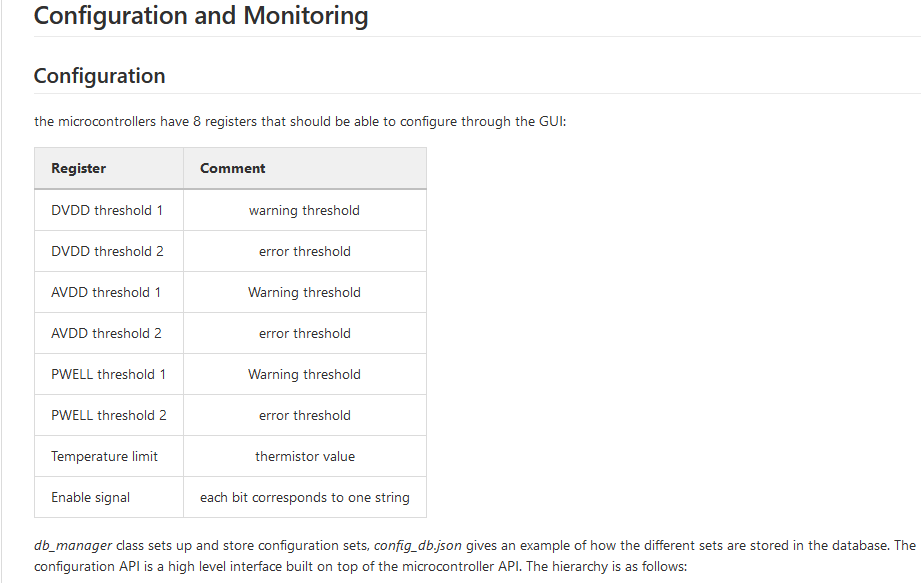
\includegraphics[width=18cm]{images/README_example.png}
    \caption{Example from the README-file showing the overview of the configuration process.}
    \label{fig: readme}
\end{figure}
\FloatBarrier

\end{document}

\end{document}